% !TEX TS-program = pdflatex
\documentclass[10pt]{article}
\usepackage{fullpage}
\usepackage{graphicx}
\usepackage{cite}
\usepackage{multirow}
\usepackage{verbatim}
\usepackage{amsmath}
\usepackage{amssymb}
\usepackage{color}
%\usepackage{hyperref}
\usepackage{lscape}
\usepackage{stackrel}
\usepackage{upgreek}
\usepackage{csquotes}
\usepackage{rotating}
\usepackage{dcolumn}
\usepackage{cite}
%\usepackage[a4paper,left=1.925cm,right=1.925cm,top=2.54cm,bottom=4.94cm]{geometry}
\usepackage[colorlinks=true, allcolors=blue]{hyperref}
\DeclareMathOperator{\spn}{span}
\renewcommand{\thetable}{\Roman{table}}
\renewcommand{\baselinestretch}{1.0} % Change to 1.65 for double spacing
\newcolumntype{d}[1]{D{.}{\cdot}{#1} }

\def\red{\textcolor{red}}
\def\blue{\textcolor{blue}}
\def\green{\textcolor{green}}
\def\magenta{\textcolor{magenta}}
\def\cyan{\textcolor{cyan}}
\definecolor{lightgray}{gray}{0.8}
\definecolor{llightgray}{gray}{0.95}


\def\##1{{\underline #1}}
\def\=#1{\underline{\underline{#1}}}
\def\+#1{\underline{\bf #1}}
\def\*#1{\breve{\bf #1}}

\newcommand{\SImu}{\ensuremath{\upmu}}
\newcommand{\SImum}{\ensuremath{\upmu}\textrm{m}}

\def\.{\mbox{ \tiny{$^\bullet$} }}


\def\le{\left(}
\def\ri{\right)}
\def\les{\left[}
\def\ris{\right]}
\def\lec{\left\{}
\def\ric{\right\}}

\def\c#1{\cite{#1}}
\def\l#1{\label{#1}}
\def\r#1{(\ref{#1})}
\def\rr#1{\ref{#1}}
\def\t#1{\mbox{\tiny{#1}}}

\def\eps{\varepsilon}
\def\epso{\eps_{\scriptscriptstyle 0}}
\def\etao{\eta_{\scriptscriptstyle 0}}
\def\ko{k_{\scriptscriptstyle 0}}
\def\lambdao{\lambda_{\scriptscriptstyle 0}}
\def\lo{(\lambdao)}
\def\lambdaoshift{\lambda_{\scriptscriptstyle 0, \rm shift}}
\def\muo{\mu_{\scriptscriptstyle 0}}
\def\alphao{\alpha_{\scriptscriptstyle 0}}
\def\co{c_{\scriptscriptstyle 0}}
\def\Eo{E_{\scriptscriptstyle 0}}
\def\lambdaomin{\lambda_{\scriptscriptstyle 0,min}}
\def\lambdaomax{\lambda_{\scriptscriptstyle 0,max}}    

\def\cpsi{\cos\psi}
\def\spsi{\sin\psi}
\def\ctheta{\cos\theta}
\def\stheta{\sin\theta}

\def\Nfs{N_{\rm f}^{\rm s}}

\def\mn{^{(m,n)}}
\def\00{^{(0,0)}}
\def\zero{^{(0)}}
\def\m{^{(m)}}
\def\n{^{(n)}}

\def\curl{\nabla\times}
\def\ux{\hat{\#u}_x}
\def\uy{\hat{\#u}_y}
\def\uz{\hat{\#u}_z}


\def\sp{\#s}
\def\pinc{\#p_{\rm +}}
\def\pref{\#p_{\rm -}}
\def\ptrs{\#p_{\rm +}}

\def\Einc{\#E_{\rm inc}}
\def\Eref{\#E_{\rm ref}}
\def\Etrs{\#E_{\rm tr}}

\def\Hinc{\#H_{\rm inc}}
\def\Href{\#H_{\rm ref}}
\def\Htrs{\#H_{\rm tr}}

\def\as{a_{\rm s}}
\def\ap{a_{\rm p}}
\def\rs{r_{\rm s}}
\def\rp{r_{\rm p}}
\def\ts{t_{\rm s}}
\def\tp{t_{\rm p}}

\def\rss{r_{\rm ss}}
\def\rsp{r_{\rm sp}}
\def\rps{r_{\rm ps}}
\def\rpp{r_{\rm pp}}
\def\tss{t_{\rm ss}}
\def\tsp{t_{\rm sp}}
\def\tps{t_{\rm ps}}
\def\tpp{t_{\rm pp}}

\def\Rss{R_{\rm ss}}
\def\Rsp{R_{\rm sp}}
\def\Rps{R_{\rm ps}}
\def\Rpp{R_{\rm pp}}
\def\Tss{T_{\rm ss}}
\def\Tsp{T_{\rm sp}}
\def\Tps{T_{\rm ps}}
\def\Tpp{T_{\rm pp}}

\def\Rs{R_{\rm s}}
\def\Rp{R_{\rm p}}
\def\Ts{R_{\rm s}}
\def\Tp{R_{\rm p}}

\def\As{A_{\rm s}}
\def\Ap{A_{\rm p}}


\def\deg{^\circ}


\def\calA{{\cal A}}
\def\calB{{\cal B}}
\def\calE{{\cal E}}
\def\calH{{\cal H}}
\def\calR{{\cal R}}
\def\calU{{\cal U}}

\def\mbbZ{\mathbb{Z}}


\def\kx{k_{\rm x}} 
\def\ky{k_{\rm y}} 
\def\kxy{k_{\rm xy}} 



\def\alphamet{\bar{A}^{\rm met}}
\def\alphasc{\bar{A}^{\rm sc}}
\def\alphatot{\bar{A}^{\rm tot}}
\def\La{L_{\rm a}}	
\def\Ld{L_{\rm d}}	
\def\Lg{L_{\rm g}}	
\def\Lm{L_{\rm m}}
\def\Ls{L_{\rm s}}
\def\LCZTSSe{L_{\rm CZTSSe}}	
\def\Lt{L_{\rm t}}
\def\da{d_{\rm a}}
\def\Lw{L_{\rm w}}
\def\Lx{L_{\rm x}}
\def\Ly{L_{\rm y}}
\def\zetax{\zeta_{\rm x}}
\def\zetay{\zeta_{\rm y}}

\def\ppol{{\textit{p}}$-$\rm polarized}
\def\spol{{\textit{s}}$-$\rm polarized}


\def\Pin{$p$-$i$-$n$}
\def\pin{\Pin~}
\def\Assc{\bar{A}^{\rm sc}_{\rm s}}
\def\Apsc{\bar{A}^{\rm sc}_{\rm p}}
\def\Asc{\bar{A}^{\rm sc}}
\def\epsw{\eps_{\rm w}}
\def\epsd{\eps_{\rm d}}
\def\epsm{\eps_{\rm m}}
\def\epsg{\eps_{\rm g}}

\def\sfE{{\sf E}}
\def\eg{\sfE_{\rm g}}
\def\ego{\sfE_{\rm g,min}}


\def\egmax{\sfE_{\rm g,max}}
\def\Ep{\sfE_{\rm p}}

\def\xio{\xi_{\rm min}}
\def\ximax{\xi_{\rm max}}

\def\Jo{J_{0}}
\def\Jomin{J_{0,min}}
\def\Jsc{J_{SC}}
\def\JscOpt{J_{SC}^{Opt}}
\def\Jph{J_{ph}}
\def\Voc{V_{oc}}
\def\Vg{V_{\rm g}}
\def\Vt{V_t}
\def\LCdS{L_{\rm CdS}}
\def\sigman{\sigma_n}
\def\sigmap{\sigma_p}
\def\Pmax{P_{max}}
\def\ni{n_{i}}
\def\Psup{P_{sup}}
\def\Nsun{N_{sun}}
\def\Voc{V_{OC}}
\def\ni{n_{\rm i}}
\def\Nc{N_{\rm c}}
\def\Nv{N_{\rm v}}
\def\Nf{N_{\rm f}}
\def\oned{^{\rm (1D)}}

\def\vth{v_{\rm th}}



\def\lambdao{\lambda_{\scriptscriptstyle 0}}
\def\lo{(\lambdao)}
\def\lambdaoshift{\lambda_{\scriptscriptstyle 0, \rm shift}}
\def\lambdaomin{\lambda_{\scriptscriptstyle 0, {\rm min}}}
\def\lambdaomax{\lambda_{\scriptscriptstyle 0,{\rm max}}}    
\def\La{L_{\rm a}}	
\def\Ld{L_{\rm d}}	
\def\Lg{L_{\rm g}}	
\def\Lm{L_{\rm m}}
\def\Ls{L_{\rm s}}
\def\LCZTSSe{L_{\rm s}}	
\def\LCdS{L_{\rm CdS}}
\def\LAZO{L_{\rm AZO}}
\def\Lt{L_{\rm t}}
\def\da{d_{\rm a}}
\def\Lw{L_{\rm w}}
\def\Lx{L_{\rm x}}
\def\Ly{L_{\rm y}}

\def\ppol{{\textit{p}}$-$\rm polarized}
\def\spol{{\textit{s}}$-$\rm polarized}

\def\As{A_{\rm s}}
\def\Ap{A_{\rm p}}
\def\Assc{\bar{A}^{\rm sc}_{\rm s}}
\def\Apsc{\bar{A}^{\rm sc}_{\rm p}}
\def\Asc{\bar{A}^{\rm sc}}
\def\alphao{\alpha_{\scriptscriptstyle 0}}
\def\alphamet{\bar{A}^{\rm met}}
\def\alphasc{\bar{A}^{\rm sc}}
\def\alphatot{\bar{A}^{\rm tot}}
\def\co{c_{\scriptscriptstyle 0}}

\def\eps{\varepsilon}
\def\epso{\eps_{\scriptscriptstyle 0}}
\def\epsw{\eps_{\rm w}}
\def\epsd{\eps_{\rm d}}
\def\epsm{\eps_{\rm m}}
\def\epsg{\eps_{\rm g}}
\def\epsdc{\varepsilon_{\rm dc}}

\def\sfE{{\sf E}}
\def\Eo{E_{\scriptscriptstyle 0}}
\def\Ei{\sfE_{\rm i}}
\def\Ec{\sfE_{\rm c}}
\def\Ev{\sfE_{\rm v}}
\def\eg{\sfE_{\rm g}}
\def\ego{\sfE_{\rm g,min}}
\def\egmax{\sfE_{\rm g,max}}
\def\EFn{\sfE_{\rm F_{n}}}
\def\EFp{\sfE_{\rm F_{p}}}
\def\Ep{\sfE_{\rm p}}
\def\etao{\eta_{0}}

\def\Jo{J_{0}}
\def\Jomin{J_{0,min}}
\def\Jsc{J_{\rm sc}}
\def\JscOpt{J_{\rm sc}^{\rm Opt}}
\def\Jph{J_{ph}}
\def\Jn{J_{\rm n}}
\def\Jp{J_{\rm p}}
\def\FF{{\rm FF}}
\def\Jdev{J_{\rm dev}}

\def\kB{k_{\rm B}}
\def\muo{\mu_{\scriptscriptstyle 0}}
\def\mun{\mu_{\rm n}}
\def\mup{\mu_{\rm p}}
\def\n0{n_{\scriptscriptstyle 0}}
\def\p0{p_{\scriptscriptstyle 0}}
\def\ni{n_{\rm i}}
\def\Nc{N_{\rm c}}
\def\Nv{N_{\rm v}}
\def\Nf{N_{\rm f}}
\def\ND{N_{\rm D}}
\def\oned{^{\rm (1D)}}
\def\RB{R_{\rm B}}

\def\Pmax{P_{\rm max}}
\def\Pin{P_{\rm in}}
\def\Psup{P_{\rm sup}}
\def\phio{\phi_{\scriptscriptstyle 0}}
\def\phip{\phi_{\rm p}}
\def\phin{\phi_{\rm n}}
\def\pin{$p$-$i$-$n$}
\def\qe{q_{\rm e}}

\def\sigman{\sigma_{\rm n}}
\def\sigmap{\sigma_{\rm p}}

\def\Voc{V_{\rm oc}}
\def\Vg{V_{\rm g}}
\def\Vext{V_{\rm ext}}




\def\Rnpz{R(n,p;z)}
\def\Rnpzrad{R_{\rm rad}(n,p;z)}
\def\RnpzSRH{R_{\rm SRH}(n,p;z)}
\def\RB{R_{\rm B}}

\def\taun{\tau_{\rm n}}
\def\taup{\tau_{\rm p}}
\def\Ln{\L_{\rm n}}
\def\Al2O3{\rm Al_{2}O_{3}}
\def\LAl2O3{L_{Al_{2}O_{3}}}
\def\LZnO{L_{\rm ZnO}}

\def\MgF2{\rm MgF_2}
\def\LMgF2{L_{\rm \MgF2}}

\def\egn{\sfE_{{\rm g},n}}
\def\ega{\sfE_{{\rm g}_1}}
\def\egb{\sfE_{{\rm g}_2}}
\def\egc{\sfE_{{\rm g}_3}}
\def\egd{\sfE_{{\rm g}_4}}
\def\ege{\sfE_{{\rm g}_5}}
\def\egf{\sfE_{{\rm g}_6}}
\def\egg{\sfE_{{\rm g}_7}}
\def\egh{\sfE_{{\rm g}_8}}
\def\egi{\sfE_{{\rm g}_9}}

\def\mLs{m_{\rm sub}}
\def\nLs{n_{\rm sub}}

\def\jth{{\rm j}^{\rm th}}
\def\egj{\sfE_{{\rm g}_j}}




\def\egn{\sfE_{{\rm g},n}}
\def\ega{\sfE_{{\rm g}_1}}
\def\egb{\sfE_{{\rm g}_2}}
\def\egc{\sfE_{{\rm g}_3}}
\def\egd{\sfE_{{\rm g}_4}}
\def\ege{\sfE_{{\rm g}_5}}
\def\egf{\sfE_{{\rm g}_6}}
\def\egg{\sfE_{{\rm g}_7}}
\def\egh{\sfE_{{\rm g}_8}}
\def\egi{\sfE_{{\rm g}_9}}

\def\mLs{m_{\rm sub}}
\def\nLs{n_{\rm sub}}

\def\jth{{\rm j}^{\rm th}}
\def\egj{\sfE_{{\rm g}_j}}


\def\Lsa{L_{1}}
\def\Lsb{L_{2}}
\def\Lsc{L_{3}}
\def\Lsd{L_{4}}
\def\Lse{L_{5}}

\def\LARC{L_{ARC}}
\def\LFTO{L_{FTO}}
\def\LITO{L_{ITO}}






\renewcommand{\thefootnote}{\fnsymbol{footnote}}



\begin{document}

\begin{center}

\LARGE{ {\bf Solar Cell Simulator User Manual v1
}}
\end{center}
\begin{center}
\vspace{10mm} %\large

Faiz Ahmad
Akhlesh  Lakhtakia, and Peter B. Monk\\
{Send queries: monk@udel.edu}\\
\normalsize

 
\end{center}
\section{Introduction}
Welcome to the Solar PV Simulator! This software enables users to simulate the behavior of a solar cell under various conditions. By adjusting input parameters such as the thickness of different layers, bandgap energies, and material properties, users can explore how these factors influence solar cell performance. Detailed information on the optoelectronic model and material properties can be found in Refs.~\cite{Anderson2020, SolCellBook, Ahmad2022-2}. Schematic of the CIGS solar cells is provided in Fig.~\ref{Fig1}.


%%%%%%%%%%%%%%%%%%%%% Figure 1 begins %%%%%%%%%%%%%%%%%%%%%%
\begin{figure}[h] 
	\centering   
	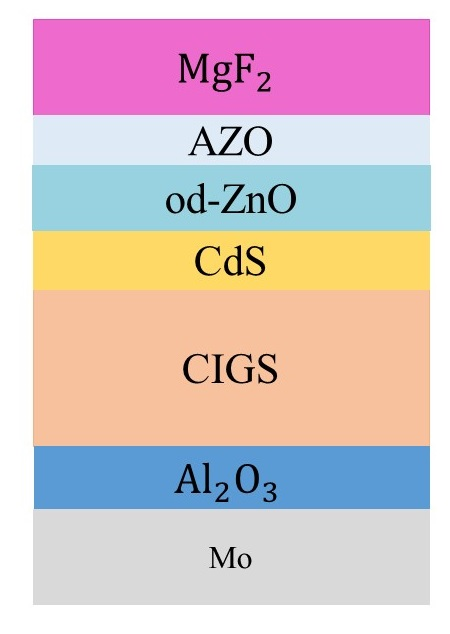
\includegraphics[width=0.4\columnwidth]{CIGS-Schematic} 
	\caption{ Schematic of a CIGS thin-film  solar cell.
		\label{Fig1} }
\end{figure}
%%%%%%%%%%%%%%%%%%%%% Figure 1 ends %%%%%%%%%%%%%%%%%%%%%%


\section{Installation}
Install MATLAB R2020b or later. Ensure MATLAB is installed and properly licensed.

\section{Getting Started}
Download the Simulator: Download the SolarCellSimulator
from GitHub by cloning \href{https://github.com/nibj/SolarCellSimulator.git} .Inside the folder locate and
open RunSimCIGS.m in the Matlab command prompt.


\section{RunSimCIGS.m}
The simulation is configured for standard CIGS solar cells and offers a simple interface to input the thickness of the CIGS photon-absorbing layer. The thickness, denoted as $\Ls$, can be specified between $100$~nm and $2200$~nm. Additionally, you can set the bandgap of the CIGS photon-absorbing layer, represented as $\ego$, within the range of $0.947$~eV to $1.626$~eV. This simulation can be adapted for different compound semiconductor solar cells (such as CZTSSe, CeTeSe, and perovskites) and their parameters need to be modified. To modify the simulation, the files \emph{DesignJunctionCIGSRunSim.m} and \emph{DesignSimCIGSRunSim.m} must be updated.

\subsection{DesignJunctionCIGSRunSim.m}
Three structures are created. 

\subsubsection{Input}
This step sets the initial values for the grating periods $\Lx$, grating height $\Lg$, solar concentration (number of suns, $\Nsun$), external voltage (keep it at 0), and the generation rate. The generation rate can be specified as a single number (for constant generation everywhere), an array of numbers with a length matching the number of electrical sections (refer to \emph{sim.material.elecsec}), or as a function. Use \emph{-inf} if the generation rate is calculated using the rigorous coupled wave approach (RCWA).
  

\subsubsection{Material}
Design the baseline properties of the device here. Specify the total number of layers for the simulation and their respective properties. Include sections for the periodic region and electrical calculations. Ensure that \emph{nsec} matches the lengths of each array specified. Single entries will be internally duplicated to this length (i.e., constant everywhere).

Periodic sections, such as the grating, are specified using the following format:
\begin{verbatim}
	'periodicsec', [0,0,0,0,0,1,0], ...
\end{verbatim}
In this example, the penultimate section is periodic. When material data is loaded (see below), the material specified is the one closest to the edge of the domain. Periodic section details are loaded from \emph{periodic} (see below).

Inputs that take strings must contain \emph{nsec}-1 '\&' symbols to distinguish between sections. For example, the line
\begin{verbatim}
	'material', 'Air & AZO & od-ZnO & CdS & CIGS & Al2O3 & Mo' , ... 
\end{verbatim}
instructs the model builder to load the material properties for air for the 1st section, AZO for the 2nd, and so on. This will overwrite the specified parameters below if those parameters are in the data file. For user-entered properties, specify the section material as 'User' to use the values specified below. For string input, spaces around the '\&' do not matter, but capitalization does.


\subsubsection{Periodic}
The number of entries in \emph{nx\_sec} must match the number of section flagged to be periodic in \emph{sim.material.periodic}.

Periodic sections can either be specified using a surface function $g(x)$ or a width function $f(z)$. Note that only periodic sections with a single protrusion are implemented, e.g. a square grating, or a bump, and so only a single period can be simulated.

For \emph{zeta} it is possible to specify a constant, e.g. 0.5 creates a square grating with 0.5 duty cycle, or a function, e.g. \emph{'@(z) (1/pi) * acos(z/80)'} creates a sinusoidal grating when Lg = 80. Notice that the input, z, is scaled to run from 0 to 1, while the output is also scale from 0 to 1. With \emph{relief}, it is possible to specify the surface, e.g. \emph{'@(zeta) cos(2*pi*zeta)'} also creates the same sinusoidal grating. Toggle between these options with \emph{zr\_flag}.


\subsection{DesignSimCIGSRunSim}
Most components are clearly labeled in this section. Two structures are created: one for setting up the optical simulation and one for the electrical simulation. The variables \emph{optical\_toggle} and \emph{electrical\_toggle} are used to turn the respective sections of the simulation off (0) or on (1).

\subsubsection{Optical}
Simulation parameters for the optical calculation are specified here. The number of entries in \emph{nslices} must match the number of sections set in \emph{DesignJunctionCIGSRunSim}. Additionally, specify the range of free-space wavelengths (minimum and maximum) for the simulation.
 
\subsubsection{Electrical}
Simulation parameters for the electrical calculation are specified here. The number of entries in \emph{nx\_sec} must match the number of sections designated as electrical in \emph{DesignJunctionCIGSRunSim} (see \emph{sim.material.elecsec}).

\subsection{Functional Inputs}
Scaling for functional inputs should be played with to make sure the domains and ranges are correct. Where a function is supplied the domain is 0 for one side of the section, to 1 at the other side of the section. Multiple functions are specified as e.g. \emph{'@(z) cos(2*pi*z) \& @(z) z + 1'}. This again should match the number of required sections.


\subsection{Make Material}
The material make files are stored in folder \emph{Materials}. These construct the data files which are loaded when a material is loaded. To add a new material, keep to the same format as those provided. If information is not provided, the user specified value will be used. To catch if this is the case, may be good to set user specified to nan. To load the data, use the generated .mat file name as the material name.




\section{Running a Simulation}
\textbf{Run Simulation:} Click the "Run" button.\\
\textbf{Enter Parameters:} You will be prompted to enter the thickness of the CIGS photon absorbing layer. The thickness, denoted as $\Ls$, can be entered in the range of $100$~nm to $2200$~nm. Following this, you will be prompted to input the bandgap of the CIGS photon absorbing layer. The bandgap, represented as $\ego$, can be entered in the range of $0.947$~eV to $1.626$~eV. \\
\textbf{View Results:} Efficiency ($\eta$), short-circuit current density ($\Jsc$), open-circuit voltage ($\Voc$), and $\FF$ output will be displayed. The IV curve will be plotted.\\
\section{Interpreting Results}
\textbf{$\Jdev$-$\Vext$ Curve:} The graph shows the relationship between current and voltage for the solar cell.\\
\textbf{Efficiency:} Indicates the percentage of power converted from absorbed light to electrical energy.\\
\textbf{$\Jsc$:} Indicates the solar cells maximum current density that can be extracted from a solar cell under short circuit conditions.\\
\textbf{$\Voc$:}  Indicates the maximum voltage that can produce across the solar cell when its terminals are open and there is no current.\\
\textbf{$\FF$:} Indicate the quality of the solar cell i.e., the ratio of maximum obtainable power to the product of $\Jsc$ and $\Voc$. 

\section{Contact and Support}
For further assistance, please contact at Email: monk@udel.edu. 
Thank you for using the Solar PV Simulator!

\newpage
\begin{thebibliography}{99}

\bibitem{Anderson2020}
T. H. Anderson, B. J. Civiletti, P. B. Monk, and A. Lakhtakia, ``Coupled optoelectronic simulation and optimization of thin-film photovoltaic
solar cells,''  \textit{J. Comput. Phys.} \textbf{407},  109242 (2020). \href{https://doi.org/10.1016/j.jcp.2020.109242}{https://doi.org/10.1016/j.jcp.2020.109242}.


\bibitem{SolCellBook}
F. Ahmad, A. Lakhtakia, and P. B. Monk, \textit{Theory of Graded-Bandgap Thin-Film Solar Cells} (Morgan \& Claypool) (2021). 
\href{https://link.springer.com/book/10.1007/978-3-031-02024-7}{https://link.springer.com/book/10.1007/978-3-031-02024-7}.
	
\bibitem{Ahmad2022-2}
F. Ahmad, A. Lakhtakia, B. J. Civilletti, and P. B. Monk, ``Efficiency enhancement of ultrathin CIGS solar
cells by optimal bandgap grading. Part II: finite-difference algorithm and double-layer antireflection coatings,"
{Appl. Opt.} {\bf 61},  10049--10061 (2022). \href{https://doi.org/10.1364/AO.474920}{https://doi.org/10.1364/AO.474920}.

\end{thebibliography}

\end{document}

